\chapter{Experimente}\label{ch:experiments}
%Auf Validität und Reliabilität achten!
Die ML-Experimente bestehen darin die Methoden praktisch umzusetzen und die Ergebnisse zu interpretieren. 
Ziel der Experimente ist einen Klassifikator zu trainieren, der den Risikoscore zuverlässig vorhersagen kann. 
Mit dessen Hilfe ist es anschließend möglich die Aktualität bzw. Richtigkeit des Scores zu überprüfen und zu aktualisieren.
Dies spart Geld, da nun nur noch die Daten aktualisiert werden müssen, bei denen der Klassifikator eine Abweichung feststellt. 
Auch für neue Kunden kann dieses Verfahren verwendet werden, um schnell ein Ergebnis zu erhalten, da nicht erst auf das Ergebnis der externen Ratingfirma gewartet werden muss.
Allerdings sollten die Daten immer aktualisiert werden und nicht nur auf den Klassifikator vertraut werden. 
Um die Datenmenge zu reduzieren, werden zunächst nur die Daten von einem bestimmten Tag geladen und analysiert.
Da die Klassifikatoren keine guten Ergebnisse aufweisen, wird als Lösung ein Upsampling der Daten vorgeschlagen, das die Lücken der Labels aus älteren Daten füllt.


\section{ML-Experimente / Modell Evaluation }

\subsection{Versuchsaufbau}
Die Experimente werden auf einem Windows-Rechner in einem Jupyter-Notebook durchgeführt.
Ein Jupyter Notebook ist ein interaktives Notizbuch, in dem Pythoncode geschrieben und ausgeführt werden kann.
Visualisierungen, wie Grafiken oder Plots von mathematischen Funktionen können direkt im Dokument betrachtet werden. 
Die Vorteile liegen darin, dass verschiedene Hypothesen einfach umgesetzt und getestet werden können. 
Dies ist auch für diese Experimente sinnvoll, da unterschiedliche Parameter bzw. Ansätze getestet werden.
Das hilft dabei festzustellen, welches Verfahren mit welchen Parametern am besten eignet ist, um Daten vorherzusagen. 

%Vorteile von Jupyter Notebook
Als Python-Bibliotheken kommen pandas, numpy und sklearn zum Einsatz. 
\\
Vorgehensweise: \\


Zunächst werden die Daten mit Hilfe eines Python-Connectors von der Datenbank in das Jupyter Notebook geladen, die wie im Kapitel 3 beschrieben, durch ein Skript erzeugt werden.
%Code Exzerpt: 
Hierfür werden die Daten in ein Python-Dictionary geladen und anschließend in einer Python-Tabelle (DataFrame) gespeichert. 
Dies geschieht mit Hilfe des IBM DB2-Connectors. 
Dieses Framework ermöglicht es die Daten mit Hilfe eines SQL-Befehls direkt von der Datenbank zu extrahieren.
Deshalb können die Daten für die Experimente mit SQL von der Datenbank vorbereitet werden.%Under oversampling, train test aufteilung
Das hat den Vorteil, dass die Daten von einem Datenbankserver vorverarbeitet werden, der direkten Zugriff auf die Daten hat.
Deshalb müssen weniger Daten über das Netzwerk übertragen werden, wenn die Daten durch ein SQL eingeschränkt werden und nicht erst aus dem DataFrame in Python entfernt werden müssen. 

% was ist ein Python-Dictionary und ein DataFrame 

\subsection{Untersuchung von textuellen Daten}
In \autoref{sec:textVerfahren} werden die Möglichkeiten zur Verwendung von Rechtschreibprüfungen zur Untersuchung von Datenqualität dargestellt und erläutert.
Hierfür werden nachfolgend die Verfahren anhand des Programmcodes erläutert und beispielhaft für die Datenspalte 'Berufe' durchgeführt. 
Die Ergebnisse werden auch in dem nachfolgend beschriebenem Dashboard angezeigt, indem die Daten in einer MySQL-Datenbank gespeichert und anschließend visualisiert werden. 


Zunächst muss für die deutsche Sprache ein Wörterbuch installiert werden. 
Auf einem Linux-Rechner kann dies mit dem Befehl 'sudo apt-get install myspell-de' nachinstalliert werden. 
Für Windows muss zunächst der Ordner gefunden werden, in dem die Daten vom python-Paketmanager gespeichert werden. \cite{https://pyenchant.github.io/pyenchant/install.html}
Mit dem Python-Code 'import enchant print(enchant.Broker().describe()' kann herausgefunden werden, welche Implementierung verwendet wird, um die Rechtschreibprüfung durchzuführen.
Diese Information ist notwendig, um den korrekten Ordner in der Python-Installation zu finden. 
Für die deutsche Sprache kann das Wörterbuch igerman98 \cite{https://www.j3e.de/ispell/igerman98/} verwendet werden. %-- TODO unter gnu gpl v3 lizensiert

Um das Textfeld der Berufe zu analysieren werden diese zunächst mit dem Paket numpy, das für numerische Verfahren in python verwendet wird, aggregiert.
Dies hat den Vorteil, dass gleiche Wörter einmalig von der Rechtschreibprüfung analysiert werden müssen. 
Da es sich bei den Textdaten um Berufe handelt und es nur eine begrenzte Anzahl von unterschiedlichen Berufen gibt ist davon auszugehen, dass sich einige der Daten überschneiden. 
Der nachfolgende Programmcode zeigt die Verwendung der Funktion unique in numpy und die Konvertierung in einen Python DataFrame, der zur Weiterverarbeitung verwendet wird, vgl. \cite{https://numpy.org/doc/stable/reference/generated/numpy.unique.html}. \\


\begin{minipage}{\linewidth}
\begin{lstlisting}[language=Python,caption={Extraktion der eindeutigen Texte},captionpos=b]
 import numpy as np 
 unique, counts = np.unique(df['BERUF'], return_counts=True)
 df = pd.DataFrame(zip(unique, counts))
\end{lstlisting}
\end{minipage}


Anschließend wird die Rechtschreibprüfung auf alle einzigartigen Ausprägungen der Berufsbezeichnung angewendet und die Anzahl der Werte addiert. 
Hierfür wird zunächst das für die Sprache korrekte Wörterbuch ausgewählt. 
Um den Fortschritt der Ausführung sehen zu können, wird die Python Bibliothek tqdm %TODO bib beschreiben
verwendet. 
Anschließend wird durch die Verwendung des SpellCheckers, der in pyenchant enthalten ist, jedes Wort geprüft und im Fehlerfall auf den Zähler addiert.
Die Implementierung des beschriebenen Szenarios ist in nachfolgendem Listing zu erkennen. 
Insbesondere ist die Umsetzung der Verwendung des SpellCheckers in den Zeilen 8, 9 und 10 zu sehen. 

\begin{minipage}{\linewidth}
\begin{lstlisting}[language=Python,caption={Implementierung der Rechtschreibprüfung},captionpos=b]
 import enchant
 from tqdm import tqdm 
 from enchant.checker import SpellChecker
 
 spellChecker = SpellChecker(enchant.Dict("de_DE"))
 counter = 0
 
 for idx, row in tqdm(df.iterrows(), total=df.shape[0]):
    spellChecker.set_text(row[0])
    for err in spellChecker: 
        counter+=row[1]
\end{lstlisting}
\end{minipage}

Um den Netzwerkverkehr zu reduzieren werden nur die Daten in den DataFrame geladen, die eine Berufsbezeichnung beinhalten. 
Zur Berechnung der Gesamtzahl der verfügbaren Berufe werden mit Hilfe eines SQL Counts die Anzahl der Daten berechnet.
Der Anteil der Daten mit Rechtschreibfehler, kann durch eine Division der Wörter mit Rechtschreibfehler und der Gesamtzahl aller Wörter berechnet werden und liegt bei knapp 24\%. 


Das Ergebnis dieser Berechnung muss nun für die Visualisierung in einer Datenbank gespeichert werden, damit diese darauf zugreifen kann. 
Hierfür wird ein Python Skript verwendet, das die Berechnung durchführt und anschließend mit einem SQL Insert in der Datenbank speichert. 
Das Python Skript kann entweder mit Hilfe eines Cron Jobs einmal pro Nacht ausgeführt oder in die Jobsteuerung des DataWarehouse integriert werden.


Es sind in den berechneten 24\% fehlerbehafteten Daten auch Fehler enthalten, die darauf zurückzuführen sind, dass die Rechtschreibprüfung Abkürzungen wie z. B. 'techn' oder 'öfftl' nicht kennt. 
Allerdings ist es sinnvoll diese auch auszubessern, um eine bessere Datenqualität zu erreichen.
Dafür gibt es mehrere Gründe, warum dies zu einer besseren Datenqualität führt.
Zum einen kann es zu Mehrdeutigkeiten von Abkürzungen kommen, die zu Fehlern führen, weil die wahre Bedeutung unterschiedlich interpretiert werden kann. 
Zum anderen können für das gleiche Wort mehrere Abkürzungen verwendet werden, wie z. B. 'öff.', 'öfftl.', 'öffentl.'.
Wenn für die gleiche Bedeutung eines Wortes mehrere Abkürzungen vorhanden sind, ist es schwieriger diese auszuwerten.
Möchte man alle Personen, die im öffentlichen Dienst arbeiten aus den Daten extrahieren, so müsste man in diesem Datensatz alle denkbaren Abkürzungen bei der Abfrage mit angeben. 




\subsection{Erzeugen der ABT und Erstellen eines Data Quality Reports}

\subsection{Datenaufbereitung }
Zunächst werden die Daten genauer untersucht, um festzustellen ob die Daten bereinigt werden müssen oder ob sich die Klassenverteilung zu sehr unterscheidet. 
Zunächst zeigt eine Grafik die Verteilung der einzelnen Klassen. 
In der Abbildung ist zu erkennen, dass die Klassen sehr ungleichmäßig verteilt sind.

Klasse 0E ist deutlich häufiger vertreten als die anderen Klassen. 
Dies führt für einige Verfahren zu Problemen und sollte behoben und vor allem durch die Verwendung von geeigneten Metriken beobachtet werden.


%---------------------- Todo EVTL in neues Kapitel verschieben 
Außerdem sind in dem vorliegen Datensatz einige textuelle Attribute.
Diese können durch einen OneHot Encoder so aufbereitet werden, dass sie in einem Klassifikator verwendet werden können.
Das Feld 'BERUF' besteht aus Berufen, die von den Bankmitarbeitern eingetragen werden.
Da die Berufsbezeichnung nicht genderneutral notiert sind, wird mit Hilfe eines Stemmings die Daten auf eine gemeinsame Grundform überführt.
Hierbei wird der Snowball Stemmer von NLTK verwendet, da dieser auch für die Deutsche Sprache geeignet ist.
%----------------------

Nach einem OneHot Encoding entstehen viele Nullen in dem Datenset.
Deshalb bietet sich zur weiteren Verarbeitung eine Sparse-Matrix an.
Diese speichert nur die tatsächlich vorhandenen Daten und speichert keine Null-Werte. %Quelle

Da manche Daten sehr von anderen abweichen (Varianz sehr groß) müssen die Daten skaliert werden.
Zum Beispiel kann der Saldo einen Wertebereich von [-100.000;100.000] haben.
Die Standardabweichung ist sehr groß, da die Daten einen großen Wertebereich haben.
Aus der Formel zur Berechnung der Standardabweichung ergibt sich somit folgende Tabelle:

      | Werte bereich,      | Standardabweichung
SALDO | -100.000, 100.000   | 100.000

%Varianz ausrechnen und als Tabellenausschnitt anzeigen

Des weiteren können Daten entfernt werden, die nur einen einzigen Wert haben, da diese keinen Klassifikator trainieren können.



\subsection{Machine Learning}
\label{sub:machine_learning}
Die verwendeten Verfahren beruhen auf den in Kapitel 4 ausgewählten Methoden.
Anhand der nachfolgenden Experimente und der genauen Analyse der Daten ist zu Erkennen, dass die Klassenverteilung sehr unausgeglichen ist. 
Dies hat zur Folge, dass die gewählten Modelle zum einen nicht richtig trainiert und zum anderen nicht korrekt validiert werden können. 
Es ist deshalb wichtig die korrekten Verfahren zur Modellbewertung zu beachten.
Das heißt konkret, dass außer dem Accuracy-Score auch andere Metriken betrachtet werden müssen, wie z.B. Precision und Recall.


\textbf{Warum Undersampling?}
% Eine Baseline stellt ein einfaches Modell dar, das versucht wird zu verbessern. 
Als Beispiel zum Problem der ungleichen Klassenverteilung soll folgendes Szenario zeigen: \\
Die Klassenverteilung der Daten zeigt, dass die Klasse '0E' einen Anteil von knapp 58\% besitzen. 
Ein einfacher Klassifikator, der immer diese Klasse rät, würde somit eine Accurracy von 58\% erreichen. % TODO  \textbf{HIER NOCH DIE FORMEL EINFÜGEN}
Da Undersampling generell zu weniger Over-Fitting führt als oversampling wird zunächst versucht dieses Verfahren zu verwenden. \cite{fundamentals of ml}
%In der Liste der Klassen ist die Klasse '4A' nicht so häufig vertreten, weshalb eine Kombination der beiden Verfahren nachfolgend getestet wird. 
Das Undersampling sollte jedoch nur auf den Trainigsdaten erfolgen und nicht bevor die Daten in Trainings- und Testset extrahiert werden, da sonst die Gefahr besteht, dass das Modell nicht korrekt in der realen Verwendung funktioniert. 

% WIRD JETZT ANDERS GEMACHT Da die Daten nicht in den Arbeitsspeicher des Entwicklungsrechners passen wird die Funktionalität des Train / Testsplit zunächst in SQL geschrieben, damit dies von dem Datenbankserver übernommen werden kann, der genügend Ressourcen zur Verfügung hat. 



\textbf{Aufteilen in train/validation/test}
Um ein Overfitting zu vermeiden und auch erkennen zu können bietet sich die Aufteilung der Daten in drei Kategorien an.
Der größte Anteil wird für das Training verwendet.
Zusätzlich zu einem test-Datensatz wird allerdings noch ein Validierungs-Datensatz extrahiert.
Dieser Datensatz wird während der Parameteranpassung nicht verwendet und so kann anhand diesen Datensatzes erkannt werden, wie gut sich das Modell bei neuen, ungesehenen Daten verhalten würde. 
Typische Größen zur Aufteilung liegen bei 50:20:30 oder 40:20:40. 
In diesem Projekt wird der Split bei 50:20:30 gesetzt, um einen möglichst großen Anteil an Daten für das Training zur Verfügung zu haben. 
\cite{Fundamentals of ML Kapitel 8}
In konkreten Zahlen bedeutet das eine Aufteilung in 60.000, 24.000 und 36.000. 
%67.257, 26903, 40354
Da die Daten zur Validierung nicht während des 

%Jedes Verfahren wird mit Upsampling brauchbar gemacht.
%Warum? (grob: was ist upsampling / oder Kapitel 4 verweisen)
%Wie wird das Upsampling gemacht?

\textbf{Erstellen einer Baseline}
https://datascience.stackexchange.com/questions/30912/what-does-baseline-mean-in-the-context-of-machine-learning

Zunächst wird für die Durchführung der Machine Learning Experimente ein Modell erzeugt, dass auf eine primitive Weise das Problem löst.
Dadurch kann mit einem Ansatz verglichen werden und in den Experimenten ist erkennbar, ob die neu gewählten Modelle besser als der naive Ansatz sind. %\cite{https://developers.google.com/machine-learning/glossary#baseline}
Ziel ist es einen Klassifikator zu definieren, der besser als das einfache Modell ist. 
Ein baseline Ergebnis bezeichnet die einfachste mögliche Vorhersage. 
Bei einem Klassifikationsproblem kann beispielsweise als Vorhersage immer die am häufigsten vertretene Klasse verwendet werden. \cite{brownlee2014}
Mit Hilfe einer Baseline kann durch Vergleiche herausgefunden werden, ob die Verwendung von anderen Attributen oder einem anderen Klassifikator bessere Ergebnisse liefern. \cite{brownlee2014}

Ein Baseline Modell kann mit Hilfe des DummyClassifiers von sklearn erzeugt werden. 
Dieses kann mit Hilfe von verschiedenen Strategien ein einfaches Modell definieren und dessen Performance getestet werden. %siehe https://scikit-learn.org/stable/modules/model_evaluation.html#dummy-estimators

Es werden verschiedene Baseline Modelle getestet und das beste für die weiteren Vergleiche verwendet. 
Dieses wird mit dem Parameter 'most\_frequent' erreicht und hat eine Accuracy von 55\% und eine Precision von 31\%. 

\textbf{Ergebnisse aus den vorgestellten Verfahren}
Für die einzelnen Klassifikatoren, die in \autoref{ch:methods} definiert und beschrieben sind, werden die Experimente nachfolgend durchgeführt.
Hierfür werden die Parameter angepasst, die die Klassifikatoren definieren. %Evtl wird hier auch mit RandomizedSearchCV getestet
Des weiteren werden Datenverbesserungen, wie Scaling und das Entfernen von Outliers getestet. 
Die Ergebnisse werden nachfolgend aufgelistet und das beste der Ergebnisse abschließend beschrieben. 
Als Vergleich soll das Baseline Modell dienen, das im vorherigen Abschnitt definiert ist.



\begin{tabular}[h]{l|c|c|c}
Klassifikator & Accuracy        & Precision & Scaler \\ \hline
Baseline & 0.55 & 0.31 & Standard Scaler \\
KNN & 0.583 & 0.464 & Standard Scaler \\
RandomForest & 0.544 & 0.55 & Standard Scaler \\


Baseline & 0.55 & 0.30 & Kein Scaler \\
KNN & 0.565 & 0.43 & Kein Scaler \\
Random Forest & 0.63 & 0.57 & Kein Scaler \\

\end{tabular}




KNN
- trainieren
    - Mit / Ohne Upsampling
    - Mit gleicher / ungleicher Klassenverteilung
    - unterschiedliche K - Werte
- Modell Bewerten 
    - train dev test
    - f1-score, accuracy und precision
    - stratified k-fold cross validation
    - f1-score, accuracy und precision 

    
SVM
- trainieren
- Modell Bewerten 
    - train dev test
    - f1-score, accuracy und precision
    - stratified k-fold cross validation
    - f1-score, accuracy und precision 

Random Forest
- trainieren
- Modell Bewerten 
    - train dev test
    - f1-score, accuracy und precision
    - stratified k-fold cross validation
    - f1-score, accuracy und precision 


Zusammenfassung: Welcher hat das beste Klassifikationsergebnis?
In diesem Kapitel wurden die Verfahren KNN, SVM, blabla getestet und der beste Klassifikator ist blabla.

\subsection{Evaluation der Machine Learning Modelle}
\label{sub:evaluation}



%Scoringverfahren:



%Was sind Daten die Einfluss auf das Kundenrating haben?
%-> Für welche Daten wäre es besonders wichtig die Datenqualität händisch zu überprüfen


%ML-Verfahren, immer inklusive Performance-Grafik:
%- logistische Regression


%Ziele:
%- Vorhersagen des Risikoscorings anhand der Inputdaten

%Aufbau:
%- python als Programmiersprache
%- Aufteilen in train-dev-test
%- 


%\subsection{KNN}

%Variabilität (Einfluss der Parameter auf das Ergebnis):
%- verschiedene k-Werte 
%- Manhattan vs. Euklidische Distanz


%\subsection{SVM (Multiklassen)}

%Verschiedene Parameter:
%- unterschiedl. Kernelfunktionen
%- C-Parameter, der über Slackvariablen gesteuert wird
%- 

%- Neuronale Netze

%- Classifikation Tree



%Aufbau Experimente: 
%Ziele*ʹ Aufbau*ʹ Ergebnisse*' Interpretation*ʹ Threats*to*Validity
%(Seite 93 https://userpages.uni-koblenz.de/~laemmel/esecourse/slides/perf.pdf)


%Ideen:
%- Komplexe Funktionen mit Stakeholdern basteln, zb wenn verheiratet dann Alter > 18
%- Daten für zb Aktualität müssen definiert werden, ob sie beispielsweise überhaupt verfallen können. Zb Geburtsdatum ändert sich nie; Alter schon
%- Ist es möglich solche Regeln mit HIlfe von ML abzuleiten oder funktioniert das gar nicht? 
%- Daten vor einem Monat berechnen, wie viele sich ändern müssten (aufgrund von zb Timeliness, correctness) und dann nachschauen wie viele sich tatsächlich geändert haben
%- Big Data Quality A Quality Dimension evaluation hat zwei konkrete Experimente, dort kann man sich gute Ideen holen. Es wird auch ein Experte zu Rate gezogen, der beispielsweise angibt, welche Daten gelöscht werden können (zb wenn 80\% der Attribute fehlen). Es hat auch einige Visualisierungen 
%- Mit SQL: 
%https://dataform.co/blog/advanced-data-quality-testing




%Auf die verschiedenen Ebenen Aktualität, Richtigkeit, Vollständigkeit und Konsistenz eingehen!
%Oft ist es besser die Daten nachzufordern, anhand eines möglichen Fehlers kann nicht der Originalzustand wiederhergestellt werden

%\section{Visualisierung}

%https://www.elastic.co/guide/en/kibana/6.8/createvis.html

\subsection{Visualisierung}
\label{sub:visualisierung}
Damit die Daten für die Visualisierung verfügbar sind, müssen diese zunächst in das Visualisierungstool integriert werden. 
Da zur Erstellung des Dashboards das Tool Grafana vorgeschlagen und verwendet wird, müssen die Daten an Grafana angebunden werden.

Wie bereits erwähnt, ist es zwar sinnvoll einen Konnektor zu verwenden, allerdings gibt es keinen Konnektor zwischen Grafana und der DB2 Datenbank.  \\

Folgende Lösung zur Integration der Daten wird im Projekt stattdessen verwendet. 
Die Daten werden mit Hilfe der DB2-Exportfunktionalität exportiert und als CSV-Datei gespeichert. 
Diese Datei wird anschließend mit Hilfe von SQL in eine MySQL Datenbank exportiert. 
Um die Daten regelmäßig zu migrieren kann ein Cron-Job verwendet werden, der beispielsweise einmal in der Nacht ausgeführt wird. 
In Zukunft kann das ETL-Tool, mit dem die Daten aus den Quellsystemen gesammelt und aggregiert werden, verwendet werden, um die Daten direkt in die MySQL Datenbank zu exportieren.
Da dieses Tool eine Steuerung zur automatischen Ausführung von Programmen beinhaltet ist es möglich den Export dort zu hinterlegen und es ist kein Cron-Job mehr nötig. 

%Verweis auf Grafana Kapitel



\textbf{Untersuchung der Dimension Richtigkeit} \\
Anhand der Analyse der Daten in einer Zeitreihe, kann erkannt werden, ob in bestimmten Zeiträumen auffällig viele bzw. wenige Datensätze vorhanden sind. 
Mit Hilfe der Visualisierung lassen sich auffällige Tage erkennen, die nicht dem Muster entsprechen. 
Dabei ist allerdings nur auf einer abstrakteren Ebene zu erkennen, ob es ein Problem in der Datenverarbeitung gegeben hat. 
Beispielsweise ist nicht zu erkennen, ob sich eine Datenreihe von einem konkreten Konto besonders auffällig verändert hat, da diese Analysen in dieser gruppierten Darstellung untergehen. 

Zunächst werden für eine Untersuchung die Daten jeweils nach dem aktuell gültigem Datum gruppiert und der aktuelle Saldo summiert.
Dies wird als SQL-Befehl in Grafana in einem neuen Dashboard bzw. Panel hinterlegt.
An der rechten Seite kann die Visualisierung ausgewählt und farblich angepasst werden.
Des weiteren muss der richtige Zeitraum ausgewählt werden, sodass die Daten angezeigt werden können.

\begin{figure}[h]
\centering
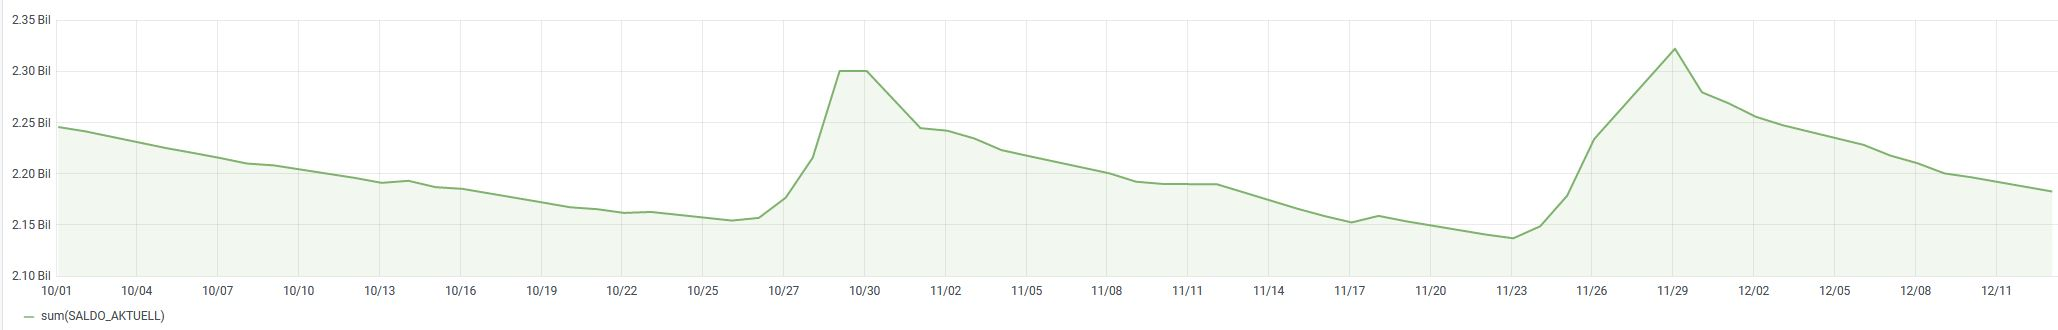
\includegraphics[width=150mm,scale=1]{content/Saldo_aktuell.jpg}
\caption{Visualisierung der Veränderung des Saldos}%
\end{figure}


In der Grafik ist ein eindeutiges Muster zu erkennen. 
Bei der Analyse von drei Monaten ist zu sehen, dass immer zum Ende bzw. Anfang des neuen Monats der Gesamtsaldo aller Konten besonders hoch ist. 
Dies ist vermutlich damit zu erklären, dass am Anfang des Monats viele Personen ihr Gehalt erhalten und somit das Gesamtsaldo aller Konten zu diesem Zeitpunkt steigt. 
Für einen Stakeholder ist diese Information und Art der Überwachung interessant, da dieser in der Lage ist zu überprüfen, ob es Probleme mit den Prozessen zur Extraktion der Daten gegeben hat. 
Die Datenwerte sollten immer diese monatlichen Schwankungen aufweisen.
Sobald diese nicht mehr auftreten, deutet das auf ein Problem hin, das von den Stakeholdern genauer untersucht werden sollte. 
Dieses Verfahren kann von den Entwickler verwendet werden, um sie dabei zu unterstützen ihre Arbeitsergebnisse zu überprüfen.



\begin{figure}[h]
\centering
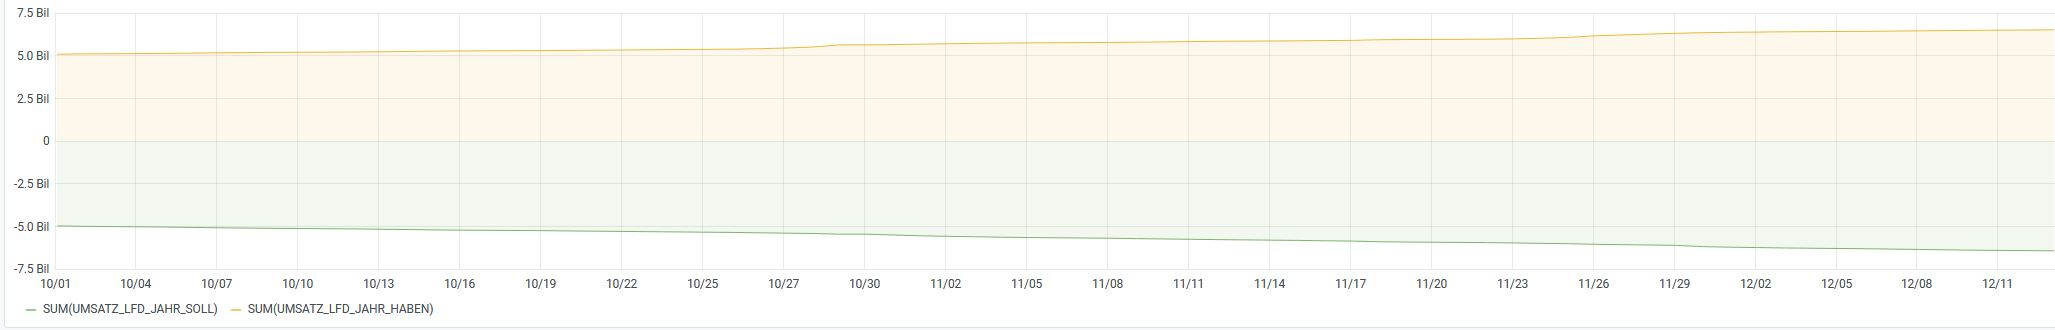
\includegraphics[width=150mm,scale=1]{content/vergleich_haben_soll.jpg}
\caption{Vergleich von Haben und Soll Umsatz}%
\end{figure}

In der Grafik ist zu erkennen, dass die Summe des Umsatzes zum Ende des Jahres generell steigen. 
Des weiteren zeigt die Datenreihe das Verhältnis des Umsatzsolls, welcher anzeigt, wie viel ausgegeben wurde. 
Da die meisten deutschen Bürger so wirtschaften, dass sie am Ende vom Jahr immer auf einen leichten Plus kommen ist zu erwarten, dass die Menge der Ausgaben insgesamt ungefähr gleich der Einnahmen ist. \cite{https://www.welt.de/wirtschaft/article189283761/Sparverhalten-der-Deutschen-Fast-jeder-Dritte-hat-am-Monatsende-kein-Geld-mehr.html}
Auch dieses Phänomen ist in der erstellten Grafik zu erkennen. 
Der negative Wert stellt den Umsatzsoll dar, dieser ist orange gekennzeichnet. 
Als Gegenpol ist in der Grafik der Umsatzhaben aufgetragen. 
Insgesamt müssen die beiden Linien sich ungefähr ergänzen. 


\textbf{Untersuchung der Dimension Vollständigkeit} \\
Um den Stakeholdern eine Möglichkeit zu geben, zu erkennen wie viele der Daten befüllt sind, bietet sich die Dimension der Vollständigkeit an.
Diese gibt an, wie viel Prozent der Datenwerte einen Wert beinhalten, also nicht null oder leer sind. 
Im vorliegenden Beispiel werden für das Dashboard die Anzahl der Kunden berechnet, die keine Berufsbezeichnung haben. 
Hierfür wird mit Hilfe eines SQLs die Gesamtzahl aller Daten, sowie der Anzahl der Daten ohne Berufsbezeichnung berechnet und anschließend geteilt. 
Einige der Daten besitzen keine Auskunft über den Beruf der Person. 
Sinnvoll wäre hier allerdings den Wert auf arbeitslos zu setzen, bei den Personen, die tatsächlich keinen Beruf haben. 
Dadurch werden die Missverständnisse aufgelöst, die entstehen, wenn eine Person als arbeitlos gewertet wird, obwohl sie einfach nur keinen Beruf angegeben hat. 
Man kann hier nicht davon ausgehen, dass die Personen keinen Beruf haben, sondern nur, dass die Daten nicht vollständig sind.









%Weitere werte die visualisiert werden, zb Anzahl der Kunden


\textbf{finden von besonders auffälligen Punkten}




\section{Diskussion zu den Dashboards}
%evtl. verschieben in ein Chapter, oder zwei mal verwenden, einmal bei Visualisierung und einmal bei ML Verfahren 
Anhand des erstellten Dashboards können die Entwickler sofort erkennen, ob durch ihre Programmänderungen, Fehler entstanden sind. 
Dies ist besonders hilfreich, da die Entwickler normalerweise nicht die gesamte Auswirkung ihrer Änderung sehen können. 
So kann die Änderung eines einzelnen Datenwertes zu Auswirkungen am Ende des Extraktionsprozesses führen, ohne dass diese direkt in der Tabelle erkannt werden, für die ein Programm angepasst wird.
Dies liegt daran, dass die Extraktionsprozesse sehr komplex sind und die Zusammenhänge der Daten nicht sofort ersichtlich sind. 
Für die Visualisierungen werden mehrere Tabellen benötigt, aus denen die Daten zusammengetragen (gejoint) werden, dadurch werden indirekt die Zusammenhänge zwischen den Daten aufgezeigt, da die Daten gesamthaft betrachtet werden. 

Auch während der Durchführung der Experimente konnte so ein Fehler entdeckt werden. 
Dieser ist dadurch aufgetreten, dass die Extraktion der Daten von DB2 als Trennzeichen ein Komma verwendet hat. 
Da die Zahlenwerte in deutscher Repräsentation abgespeichert und extrahiert werden, wird ein Komma als Dezimaltrennzeichen verwendet. 
Dieses Problem konnte erkannt werden, da die Daten des Soll-Umsatzes um ein Vielfaches von den Daten des Haben-Umsatzes abweichen. 
Die Lösung besteht darin ein anderes Trennzeichen der Datenwerte zu verwenden, das nicht in den anderen Daten vorhanden ist. 








- Data Quality Report anhand der ABT.


Integration der Daten in Kibana
- ETL Prozess zur automatischen Erzeugung einer CSV-Datei.
- Logstash?
- 

- Visualisierung von Unterschieden:
- Aggregiert nach Wochentag / Monat
- Umsatzdaten
- Kundendaten (Neukundenzuwachs?)


Kibana, Graphana

Reduktion der Datenmenge



- Welche Visualisierungen bieten sich an?
- Gibt es evtl. Visualisierungen, die DQ-Probleme aufzeigen?
